\documentclass{report}
\usepackage{inputenc} 
\usepackage{graphicx}
\usepackage{caption}
\usepackage{float}

\title{Manual for setting up the sensors of the Monitoring Box}
\author{Mick Nieman \\ Amsterdam University of Applied Sciences \and Pjotr Scholtze \\ Amsterdam University of Applied Sciences \and Heeyeon Joung \\ Seoul National University of Science and Technolgy}
\date{November 2017}

\begin{document}
\maketitle
\begin{abstract}
This has not been written yet and still needs content to be placed here. 
\end{abstract}

\tableofcontents

\chapter{Introduction}

\chapter{Requirements}
For every sensor added there is need for an Arduino Nano. The Arduino Nano is a programmable microprocessor. Advanced users may be able to connect multiple sensors to a single Arduino Nano, note that this requires advanced knowledge of the communication protocols between the Raspberry Pi 3 b+ and Arduino Nano. Along with every Arduino Nano you need an USB A to Mini-USB B cable.  \\

The first item needed for the GPS sensor is the Global Positioning System (GPS) module. We have used the Digilent 410-237 GPS-receiver board. \\

For the temperature and humidity sensor we have used the DHT22 module, this is a digital temperature- and humidty sensor. the DHT22 is more accurate (0,5$^o$ accuracy) than the previous, DHT11. It has a temperature reach from -40 to +80 $^o$C. and has a humidity reach from 10\% to 90\% with an accuracy of 2,0 \%.  \\

The heart rate sensor consists of the MAXREFDES117\# Reference Design Board with optical heart rate and pulse-oximetry monitor. It has integrated Red and Infrared LEDs. This works best on a person's fingertip or earlobe. \\

The CO$_2$ sensor comes in two varieties, the regular sensor which is affordable but less accurate and the advanced which has a higher costs and comes with higher accuracy. \\
The 'Regular CO$_2$ sensor' uses the MIKROE-1630 Daughter Board from Air Quality Click. It's an MQ-135 High sensitivity air quality sensor and potentiometer. \\
The 'Advanced CO$_2$ sensor' uses CO2meter.com its K-30 sensor. The K-30 sensor is an accurate gas sensor sensing up to 5000ppm (CO$_2$) with an accuracy of 3\%. Note that the advanced CO$_2$ meter does not work on the Arduino Nano and is only tested on the Arduino Uno. \\

The raspberry Pi Cam doesn't require to be connected to an Arduino and can be plugged directly in to the Raspberry Pi its camera-port. For this project we used Sony's IMX219 8-Megapixel Pi Camera Board. It is able for taking photographs of 3280x2464 pixels or video's at 1080p at 30 frames per second. \\

The galvanic skin response sensor, or short GSR, measures the galvanic skin response based on the electrical conductance of the skin. For the Monitoring Box we have used the Grove-GSR sensor from seeed studio.\\

Every sensor has it's own schematics for assembling the sensors, the code running on the sensor can be downloaded from https://github.com/pjotrscholtze/MonitoringBox, for the exact link for a particular sensor see further into this document.  


\chapter{Glossary}

GND pin - Ground pin \\
A1 pin - Analog pin 1


\chapter{Global Positioning System (GPS) sensor}

\chapter{Temperature and humidity sensor}

\chapter{Heartrate sensor}

\chapter{Regular carbon dioxide (CO$_2$) sensor}
The regular carbon dioxide (CO$_2$) sensor, from now on called the regular (CO$_2$) sensor, is a sensor developed by mikroelectronics, and the schematics for the assembly of the sensor are as follows. \\

\begin{figure}[H]
	\centering
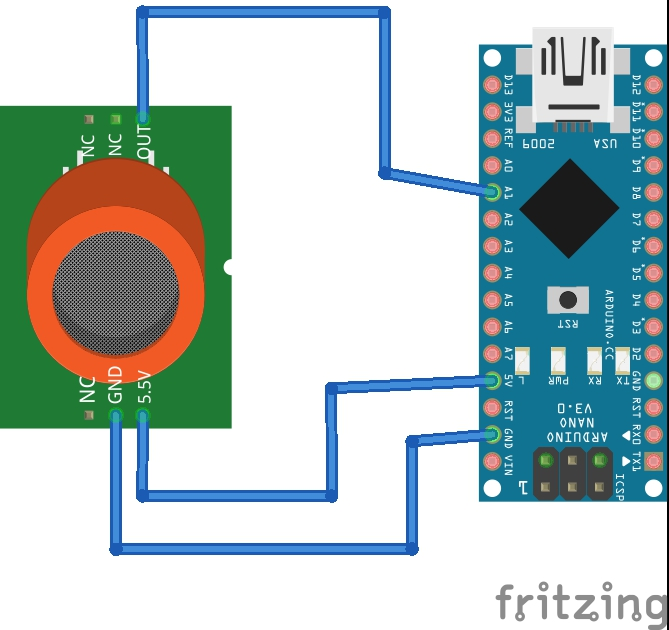
\includegraphics[width=0.75\textwidth]{images/Mikroe-Gas-sensor-schematic.jpg}
	\caption{Air Quality Click Schematic}
\end{figure}

Note that the actual sensor looks slightly different, though the pinout is the same, the 5.5V pin of the Air-quility-click goes onto the 5.5V pin on the Arduino, the GND pin on the Air-quility-click  goes onto the GND pin on the Arduino and the OUT pin on the Air-quility-click goes onto the A1 pin of the Arduino. \\
The actual sensor looks like the following:\\

\begin{figure}[H]
	\centering
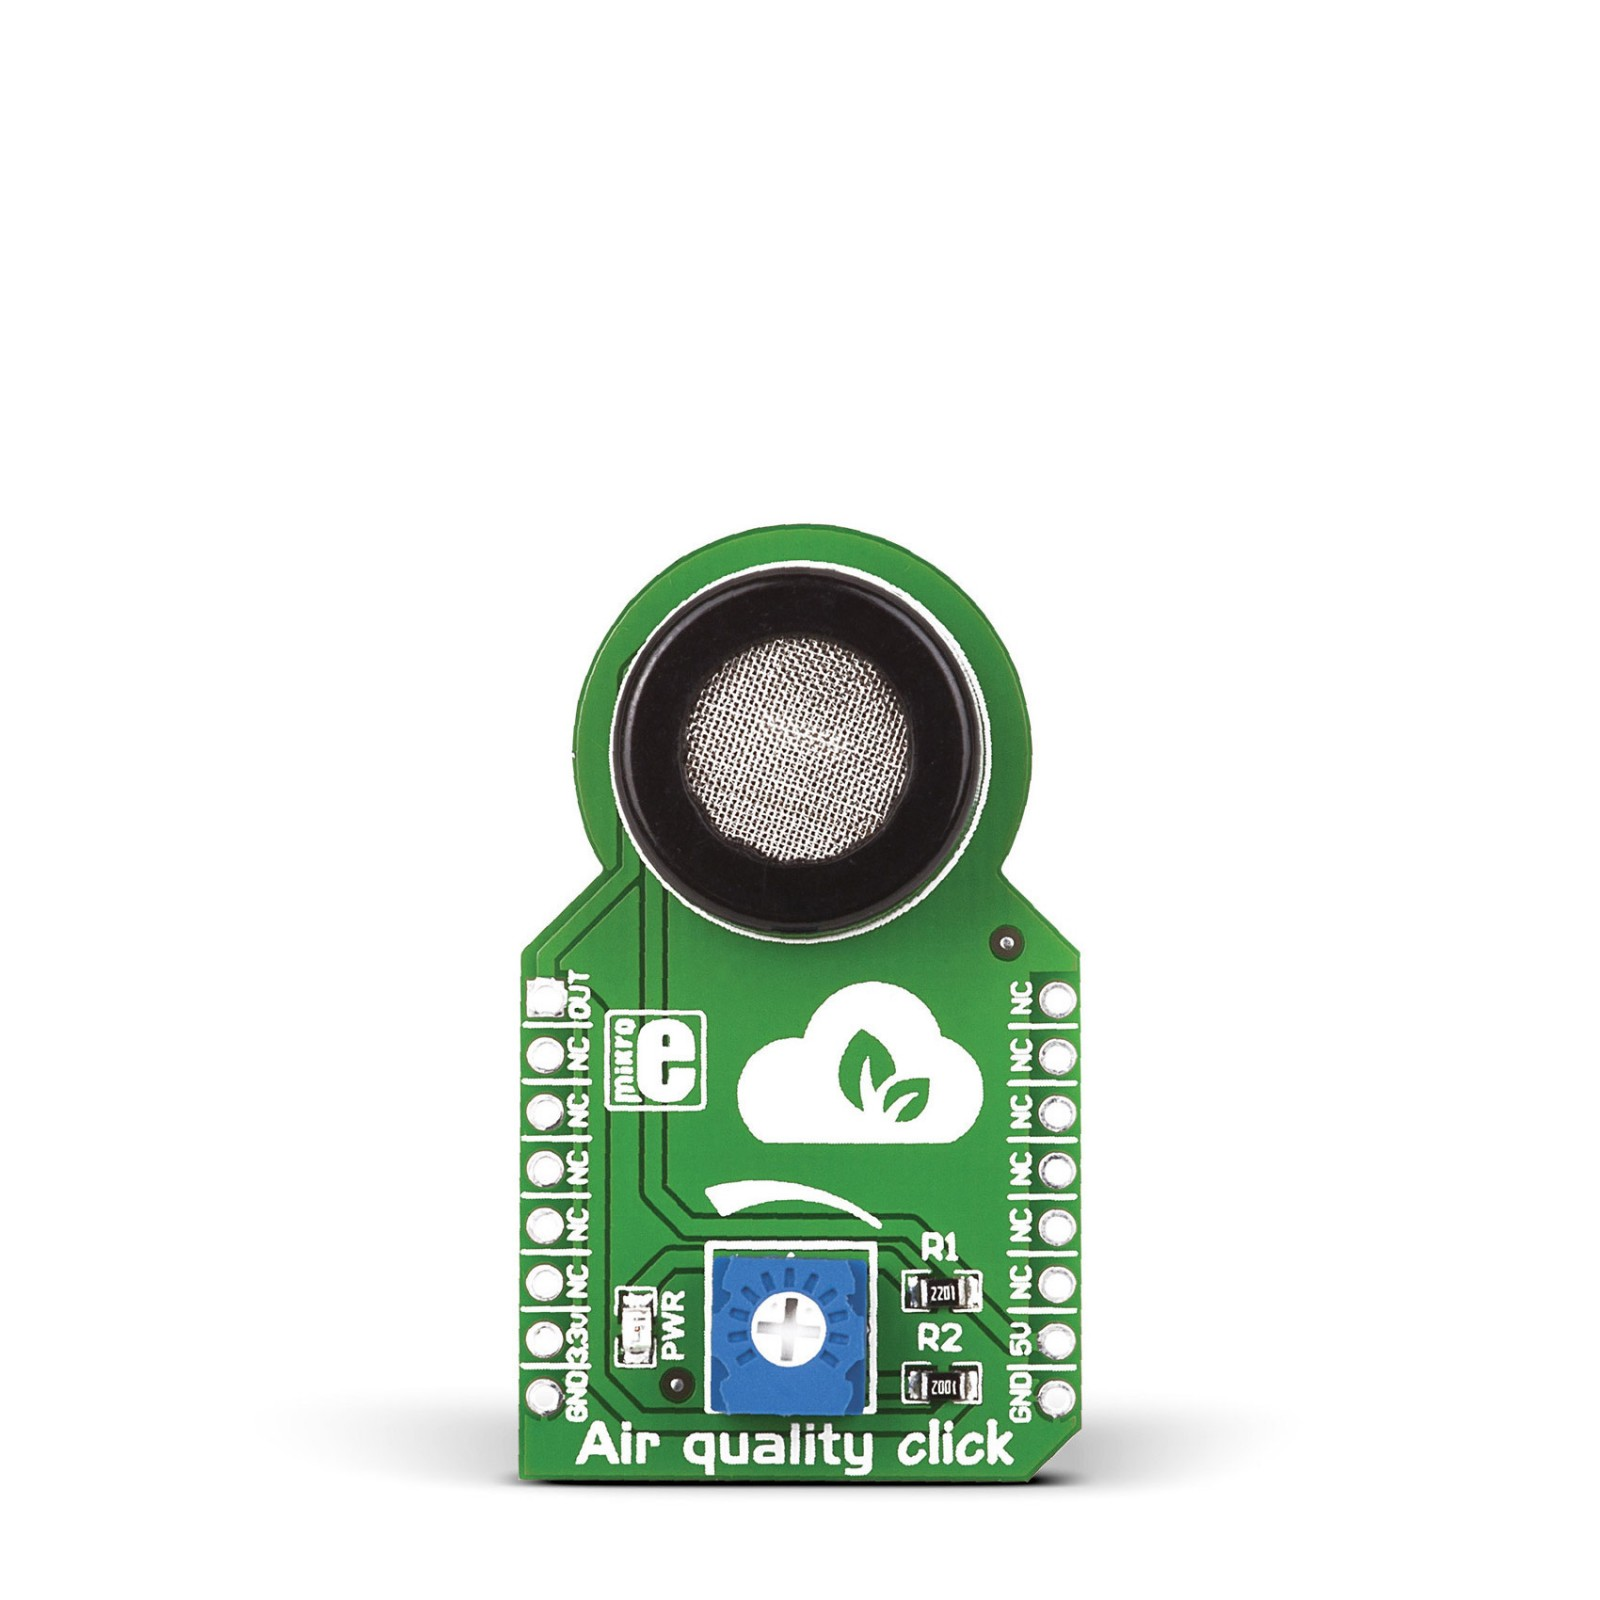
\includegraphics[width=0.75\textwidth]{images/air-quality-click-breakout.jpg} 
	\caption{The Mikroe Gas Detector}
\end{figure}

The code coming with this sensor can be downloaded with the following link: $ https://github.com/pjotrscholtze/MonitoringBox/tree/develop/Sensors/CO2\_Sensor $


Downloading the code and uploading this to the Arduino Nano and having it assembled as the schematics show should result in a functional sensor. 

\chapter{Advanced carbon dioxide (CO$_2$) sensor}

\chapter{Raspberry Pi Camera}

\chapter{Galvanic skin response sensor}

\chapter{Development issued example sensor}

\chapter{Development issued unknown sensor}

\end{document}
